\begin{figure}[t]
\small
\centering
\begin{tikzpicture}
	\draw[step=1cm, opacity=0] (-2.5,0) grid (4,0);
	\fill[black!5!white] (0,0) rectangle (4,2);
	\draw[step=1cm, double] (0,1) grid (4,2);
	\draw[step=1cm, double] (0,0) -- (0,1);
	\draw[step=1cm, double] (1,0) -- (1,1);
	\draw[step=1cm, double] (2,0) -- (2,1);
	\draw[step=1cm, double] (3,0) -- (3,1);
	\draw[step=1cm, double] (4,0) -- (4,1);
	\draw[step=1cm, dashed] (0,0) -- (4,0);
	\node (p1) at (-0.5,1.5) {$\rightarrow$};
	\node[left=-0.15cm of p1] {word $w_i$};
	\node at (2.0,3.6) {corpus of labeled documents};
	\node at (0.5,2.5) {$\downarrow$};
	\node at (1.5,2.5) {$\downarrow$};
	\node at (3.5,2.5) {$\downarrow$};
	\node at (0.5,3) {$\mathbb{D}_{c_1}$};
	\node at (1.5,3) {$\mathbb{D}_{c_2}$};
	\node at (2.5,3) {$\cdots$};
	\node at (3.5,3) {$\mathbb{D}_{c_n}$};
	\node at (0.5,1.5) {${fc_1}_{w_i}$};
	\node at (1.5,1.5) {${fc_2}_{w_i}$};
	\node at (2.5,1.5) {$\cdots$};
	\node at (3.5,1.5) {${fc_n}_{w_i}$};
	\node at (0.5,0.6) {$\vdots$};
	\node at (1.5,0.6) {$\vdots$};
	\node at (2.5,0.6) {$\vdots$};
	\node at (3.5,0.6) {$\vdots$};
\end{tikzpicture}
\begin{tikzpicture}
	\draw[step=1cm, opacity=0] (0,0) grid (1,0);
	\node at (0,1) {$\xRightarrow{\text{Group $\mathbb{P}$ and $\mathbb{N}$}}$};
\end{tikzpicture}
\hspace{-1cm}
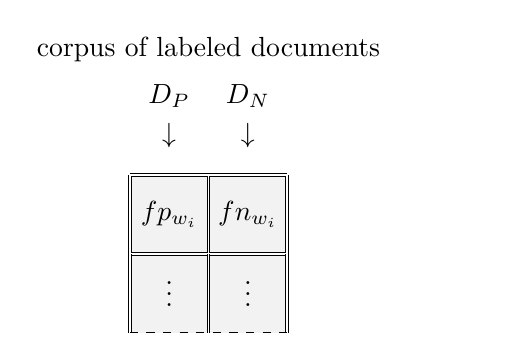
\begin{tikzpicture}
	\draw[step=1cm, opacity=0] (0,0) grid (4.5,0);
	\fill[black!5!white] (0,0) rectangle (2,2);
	\draw[step=1cm, double] (0,1) grid (2,2);
	\draw[step=1cm, double] (0,0) -- (0,1);
	\draw[step=1cm, double] (1,0) -- (1,1);
	\draw[step=1cm, double] (2,0) -- (2,1);
	\draw[step=1cm, dashed] (0,0) -- (2,0);
	%\node (p1) at (-0.5,1.5) {$\rightarrow$};
	%\node[left=-0.15cm of p1] {word $w_i$};
	\node at (1.0,3.6) {corpus of labeled documents};
	\node at (0.5,2.5) {$\downarrow$};
	\node at (1.5,2.5) {$\downarrow$};
	\node at (0.5,3) {$\mathbb{D}_\mathbb{P}$};
	\node at (1.5,3) {$\mathbb{D}_\mathbb{N}$};
	\node at (0.5,1.5) {$fp_{w_i}$};
	\node at (1.5,1.5) {$fn_{w_i}$};
	\node at (0.5,0.6) {$\vdots$};
	\node at (1.5,0.6) {$\vdots$};
\end{tikzpicture}
\caption[The frequency matrix of CopeOpi vectors]{The frequency matrix of CopeOpi vectors.\\
In the frequency matrix of CopeOpi vectors,
each row represents a unique word $w_i$ and
the $n$ columns represent $n$ corpora of labeled documents $\mathbb{D}_{c_1},\mathbb{D}_{c_2},\dots,\mathbb{D}_{c_n}$.
The element ${fc_j}_{w_i}$ is the frequency of word $w_i$
in corpus $\mathbb{D}_{c_j}$.
After $\mathbb{P}$ and $\mathbb{N}$ are grouped,
the two columns represent two corpora of labeled documents $\mathbb{D}_\mathbb{P}$ and $\mathbb{D}_\mathbb{N}$.
The elements $fp_{w_i}$ and $fn_{w_i}$ are the frequencies of word $w_i$ 
in corpus $\mathbb{D}_\mathbb{P}$ and in corpus $\mathbb{D}_\mathbb{N}$.}
\end{figure}